% fig4_states.tex —— 图 4（终端生命周期）源文件。standalone 编译：
%   pdflatex fig4_states.tex
% 2026-11-27：从 历史留档/论文改独立图前备份_20261124/main.tex.pre_export.bak 找回原 TikZ 源，
% 只改一处标签："old debt carried" → "old account carried"（模型不建模债务，见 §IV-B；
% "账户" 指 §IV-D 里链上挂的那个 account）。其余版式与原图逐字相同。
% !TeX program = pdflatex
% IEEE two-column layout (for advisor review / IEEE-family submission)
\documentclass[border=6pt]{standalone}

\usepackage[utf8]{inputenc}
\usepackage[T1]{fontenc}
\usepackage{amsmath,amssymb,amsfonts}
\usepackage{graphicx}
\usepackage{booktabs}
\usepackage{algorithm}
\usepackage{algpseudocode}
\usepackage{multirow}
\usepackage{siunitx}
\usepackage{xcolor}
\usepackage{url}
\usepackage[hidelinks]{hyperref}
\usepackage{pgfplots}
\pgfplotsset{compat=1.18}
\usepgfplotslibrary{groupplots}
\pgfplotstableset{col sep=comma}
\usepackage{tikz}
\usetikzlibrary{arrows.meta,positioning,shapes.geometric,fit,backgrounds,calc}

\sisetup{detect-weight=true,detect-inline-weight=math}

% ---- 统一样式：七个对比方法 ----
\definecolor{cOurs}{RGB}{196,30,58}
\definecolor{cLower}{RGB}{120,120,120}
\definecolor{cLeach}{RGB}{31,119,180}
\definecolor{cCfachs}{RGB}{255,127,14}
\definecolor{cAfpuck}{RGB}{44,160,44}
\definecolor{cAerdm}{RGB}{148,103,189}
\definecolor{cAfpucloc}{RGB}{140,86,75}
\definecolor{cnblue}{RGB}{31,56,100}
\definecolor{cnteal}{RGB}{46,139,139}
\definecolor{cnfill}{RGB}{240,246,246}
\definecolor{cnpale}{RGB}{226,240,240}

\pgfplotsset{
  result axis/.style={
    width=\columnwidth, height=4.6cm,
    tick label style={font=\footnotesize},
    label style={font=\footnotesize},
    legend style={font=\scriptsize, draw=none, fill=none},
    grid=major, grid style={gray!18},
    ymajorgrids=true, xmajorgrids=false,
    yticklabel={\pgfmathparse{\tick*100}\pgfmathprintnumber[fixed,precision=0]{\pgfmathresult}},
    scaled y ticks=false,
  }
}


\graphicspath{{../figures/}}
\begin{document}
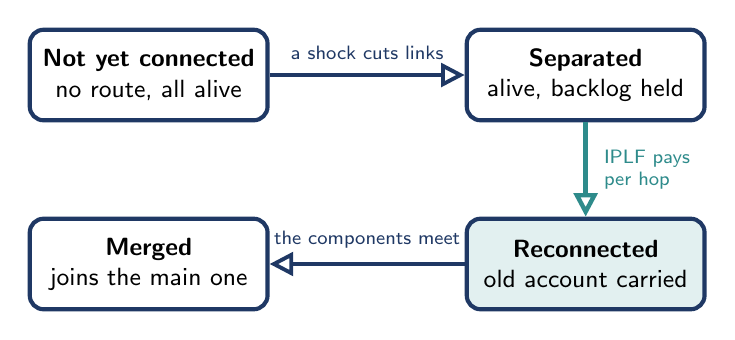
\begin{tikzpicture}[font=\sffamily\small,,
  st/.style={draw=cnblue,line width=1.5pt,rounded corners=5pt,
             minimum width=3.02cm,minimum height=1.15cm,align=center,inner sep=2pt,fill=white},
  tr/.style={-{Triangle[open,length=3mm,width=3mm]},line width=1.4pt,draw=cnblue},
  trm/.style={-{Triangle[open,length=3mm,width=3mm]},line width=1.6pt,draw=cnteal}]

\node[st] (a) at (0,2.50)    {\textbf{Not yet connected}\\ no route, all alive};
\node[st] (b) at (5.55,2.50) {\textbf{Separated}\\ alive, backlog held};
\node[st,fill=cnpale] (c) at (5.55,0.10) {\textbf{Reconnected}\\ old account carried};
\node[st] (d) at (0,0.10)    {\textbf{Merged}\\ joins the main one};

\draw[tr]  (a.east) -- (b.west) node[midway,above=1.5pt,font=\sffamily\scriptsize,text=cnblue] {a shock cuts links};
\draw[trm] (b.south) -- (c.north) node[midway,right=2.5pt,font=\sffamily\scriptsize,text=cnteal,align=left] {IPLF pays\\ per hop};
\draw[tr]  (c.west) -- (d.east) node[midway,above=1.5pt,font=\sffamily\scriptsize,text=cnblue] {the components meet};
\end{tikzpicture}
\end{document}
